\documentclass[../main.tex]{subfiles}

\begin{document}

Back before 1999, when one wanted to develop an enterprise application in Java, there was no other choice than to implement everything in Java SE. Even though Java has a relatively extensive standard library, provided abstractions were not sufficient for writing enterprise applications because application developers needed to understand these (quite) low-level abstractions upon which they could build their application.

This led to the creation and rise of Jakarta EE\footnote{Initially, its name was Java EE and was renamed once Oracle announced its submission under the Eclipse foundation.}. Citing an official Jakarta EE website: "Jakarta EE is the standard, a set of specifications for enterprise Java application development."\cite{jakartaee}. The previous sentence is short and simple, yet precisely defines what Jakarta EE is about.

Each specification is a higher-level abstraction built on top of Java SE, which can be used by application developers to develop their enterprise application without the need to understand all low-level details (this knowledge is delegated to those who implement the specification).

As an example, suppose a connection with a database has to be done from the application. We can use Jakarta Persistence specification\footnote{\url{https://jakarta.ee/specifications/persistence/}} providing more higher-level abstractions compared to abstractions provided by \textit{java.sql} package (which we would probably use from Java SE to implement database connection).

Every specification is vendor-neutral and is evolved by Jakarta EE Working Group\footnote{\url{https://jakarta.ee/about/working-group/}}, which is a global community consisting of representatives of leading technology organizations and individuals. For a visual representation of the above explanation, see Figure \ref{fig:jakarta-ee}.

\begin{figure}
  \begin{center}
    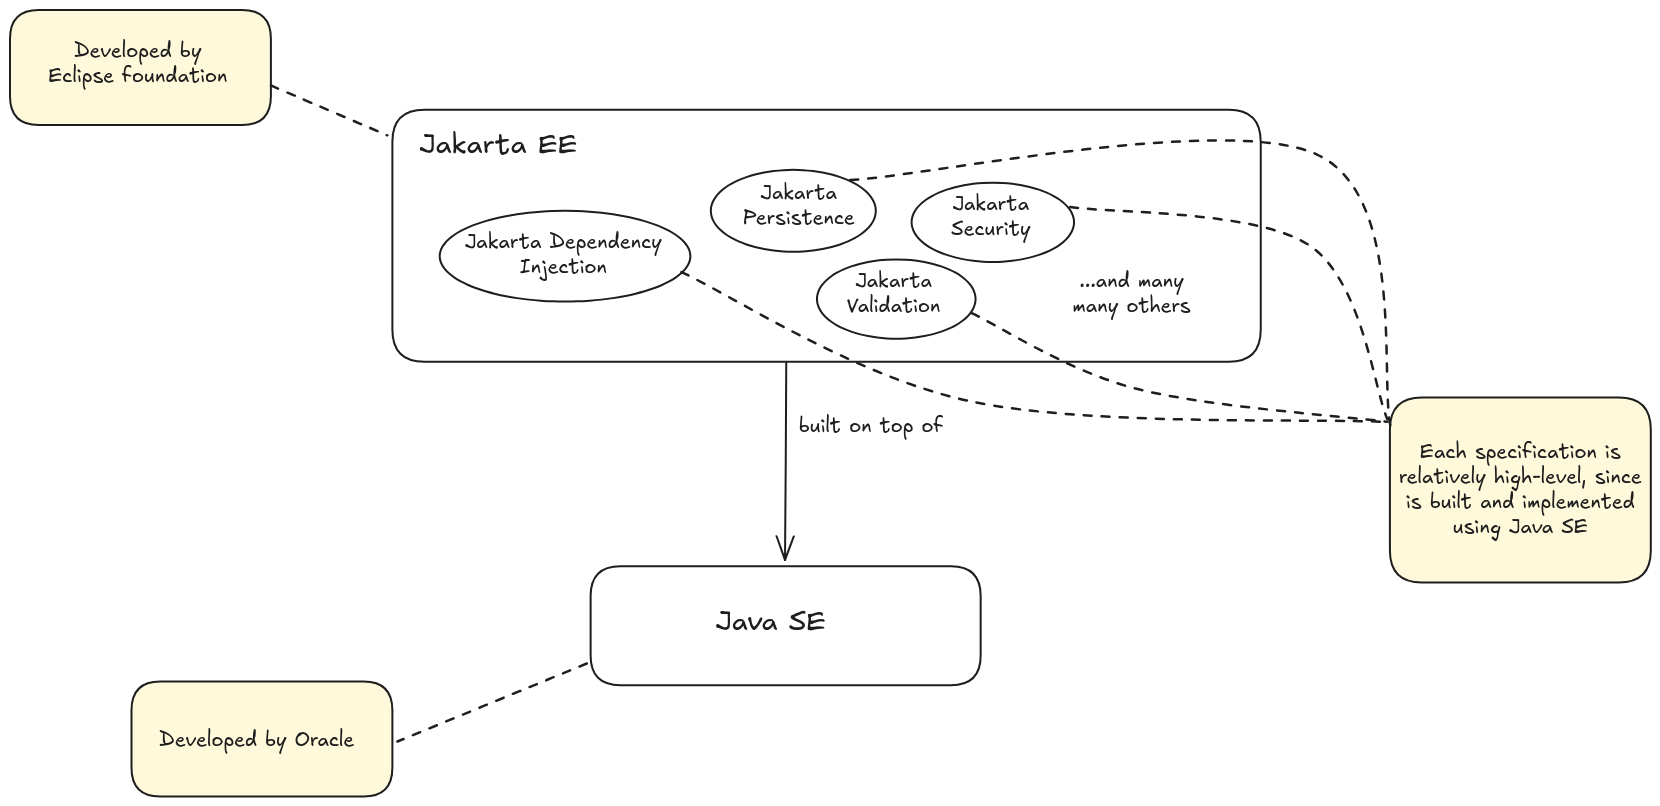
\includegraphics[width=0.7\textwidth]{images/jakarta-ee.png}
  \end{center}
  \caption{Jakarta EE building blocks}
  \label{fig:jakarta-ee}
\end{figure}

\end{document}
